\documentclass[tikz]{standalone}

\usepackage{amsmath}
\usepackage{circuitikz}

\begin{document}
    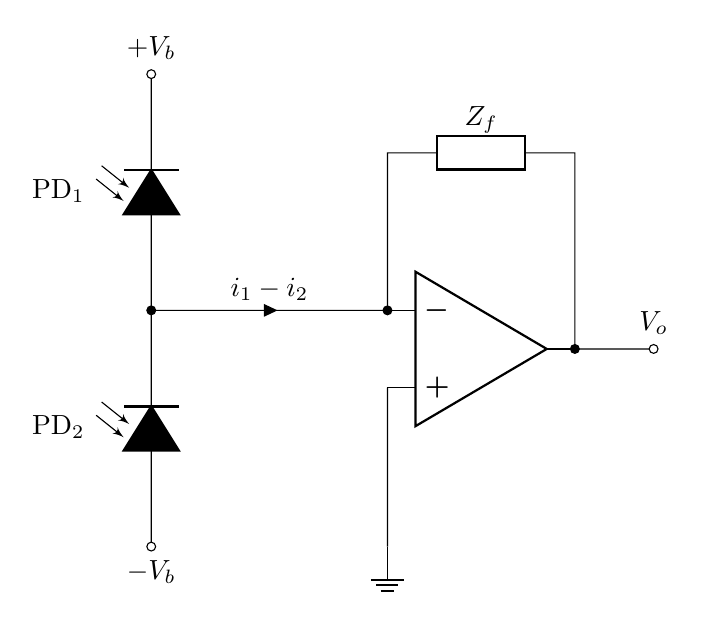
\begin{tikzpicture}
        \draw (0, 0)
            node[op amp] (opamp) {}
            (opamp.out) to ++(1, 0) node[ocirc, label=$V_o$](vout){}
            (opamp.-) node[circ](aux){} to[short, i<_=${i_1-i_2}$] ++(-3, 0) node[circ](bd){}
            (bd) to[full photodiode, l=$\text{PD}_1\;$] ++(0, 3) node[ocirc, label=$+V_b$](bias plus){}
            (bd) ++(0, -3) node[ocirc, label=$-V_b$, rotate=180](bias minus){} to[full photodiode, l=$\text{PD}_2\;$] ++(0, 3)
            (aux) to ++(0, 2) node(aux2){} to[european resistor, l=$Z_f$] (aux2 -| opamp.out) |- (opamp.out) node[circ]{}
            (opamp.+) to (opamp.+ |- bias minus) node[ground](gnd){}
            ;
%        \draw (0, 0)
%            node[ocirc, label=$-V_\text{bias}$, rotate=180]{}
%            to[full photodiode, l=PD-, i=$i_-$] ++(0, 3)
%            node[circ](bd){}
%            to[full photodiode, l=PD+, i>^=$i_+$] ++(0, 3)
%            node[ocirc, label=$+V_\text{bias}$]{}
%            ;
%        \draw (bd)
%            to[amp, i>^=${i=i_+-i_-}$] ++(6, 0)
%            node[ocirc, label=$V_\text{out}$](vout){}
%            ;
    \end{tikzpicture}
\end{document}
